\documentclass[border=10pt]{standalone}
\usepackage{tikz}
\usetikzlibrary{arrows.meta, positioning, fit, backgrounds, calc}

% Color definitions
\definecolor{uifill}{RGB}{219,234,254}
\definecolor{uiborder}{RGB}{37,99,235}
\definecolor{agentfill}{RGB}{220,252,231}
\definecolor{agentborder}{RGB}{22,163,74}
\definecolor{toolfill}{RGB}{237,233,254}
\definecolor{toolborder}{RGB}{124,58,237}
\definecolor{hwfill}{RGB}{255,237,213}
\definecolor{hwborder}{RGB}{234,88,12}
\definecolor{genfill}{RGB}{243,244,246}
\definecolor{genborder}{RGB}{107,114,128}

% Node styles
\tikzset{
  uibox/.style={draw=uiborder, fill=uifill, rounded corners=4pt, minimum height=1cm, minimum width=3cm, font=\small\sffamily, align=center, line width=0.8pt},
  agentbox/.style={draw=agentborder, fill=agentfill, rounded corners=4pt, minimum height=1cm, minimum width=3cm, font=\small\sffamily, align=center, line width=0.8pt},
  toolbox/.style={draw=toolborder, fill=toolfill, rounded corners=4pt, minimum height=1cm, minimum width=3cm, font=\small\sffamily, align=center, line width=0.8pt},
  hwbox/.style={draw=hwborder, fill=hwfill, rounded corners=4pt, minimum height=1cm, minimum width=3cm, font=\small\sffamily, align=center, line width=0.8pt},
  genbox/.style={draw=genborder, fill=genfill, rounded corners=4pt, minimum height=1cm, minimum width=3cm, font=\small\sffamily, align=center, line width=0.8pt},
  layer/.style={draw=gray!40, fill=gray!3, rounded corners=6pt, dashed, line width=0.6pt},
  layerlabel/.style={font=\footnotesize\sffamily\bfseries, text=gray!70},
  arrow/.style={-{Stealth[length=5pt]}, line width=0.7pt, color=gray!70},
  biarrow/.style={{Stealth[length=5pt]}-{Stealth[length=5pt]}, line width=0.7pt, color=gray!70},
  arrowlabel/.style={font=\tiny\sffamily, text=gray!60, midway, fill=white, inner sep=1pt},
}

\begin{document}
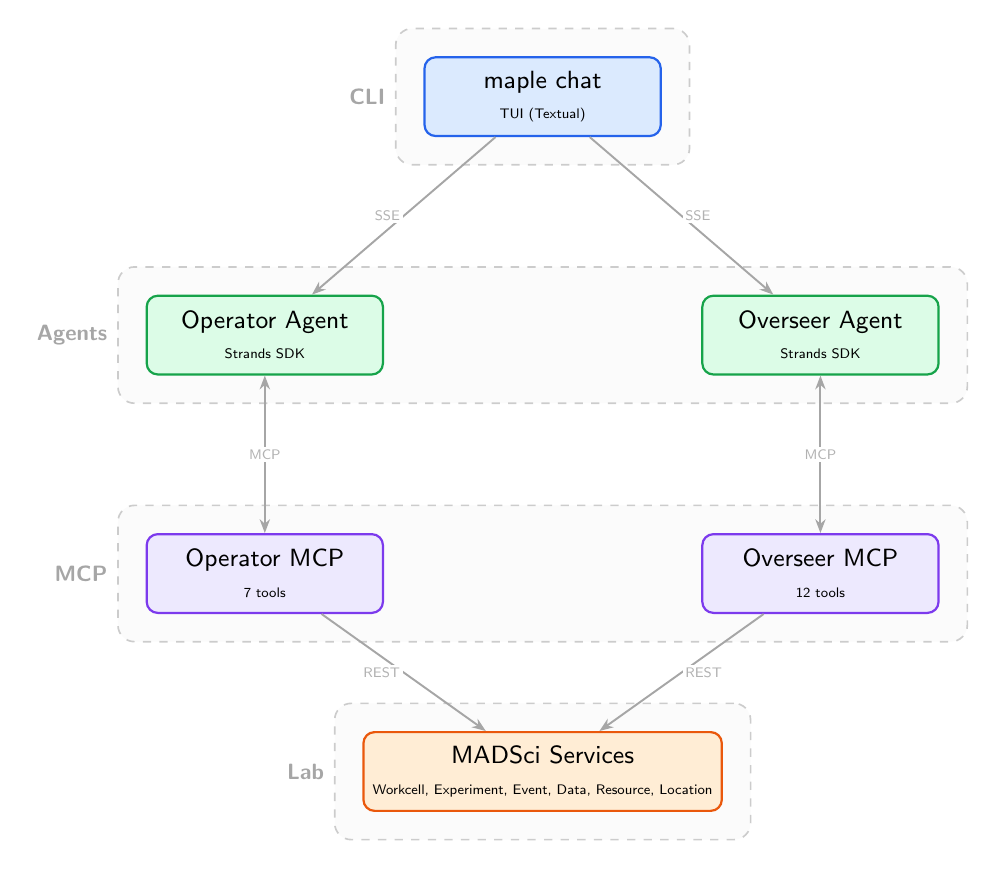
\begin{tikzpicture}

  % --- Layer 1: TUI ---
  \node[uibox] (tui) {maple chat\\{\tiny TUI (Textual)}};

  % --- Layer 2: Agents ---
  \node[agentbox, below left=2cm and 0.5cm of tui] (op-agent) {Operator Agent\\{\tiny Strands SDK}};
  \node[agentbox, below right=2cm and 0.5cm of tui] (ov-agent) {Overseer Agent\\{\tiny Strands SDK}};

  % --- Layer 3: MCP Servers ---
  \node[toolbox, below=2cm of op-agent] (op-mcp) {Operator MCP\\{\tiny 7 tools}};
  \node[toolbox, below=2cm of ov-agent] (ov-mcp) {Overseer MCP\\{\tiny 12 tools}};

  % --- Layer 4: MADSci ---
  \node[hwbox, below=2cm of $(op-mcp)!0.5!(ov-mcp)$] (madsci) {MADSci Services\\{\tiny Workcell, Experiment, Event, Data, Resource, Location}};

  % --- Layer boundaries ---
  \begin{pgfonlayer}{background}
    \node[layer, fit=(tui), inner sep=10pt, label={[layerlabel]left:CLI}] {};
    \node[layer, fit=(op-agent)(ov-agent), inner sep=10pt, label={[layerlabel]left:Agents}] {};
    \node[layer, fit=(op-mcp)(ov-mcp), inner sep=10pt, label={[layerlabel]left:MCP}] {};
    \node[layer, fit=(madsci), inner sep=10pt, label={[layerlabel]left:Lab}] {};
  \end{pgfonlayer}

  % --- Arrows ---
  \draw[arrow] (tui) -- node[arrowlabel, left] {SSE} (op-agent);
  \draw[arrow] (tui) -- node[arrowlabel, right] {SSE} (ov-agent);
  \draw[biarrow] (op-agent) -- node[arrowlabel] {MCP} (op-mcp);
  \draw[biarrow] (ov-agent) -- node[arrowlabel] {MCP} (ov-mcp);
  \draw[arrow] (op-mcp) -- node[arrowlabel, left] {REST} (madsci);
  \draw[arrow] (ov-mcp) -- node[arrowlabel, right] {REST} (madsci);

\end{tikzpicture}
\end{document}
